\documentclass{article}
\usepackage{graphicx}
\usepackage{subcaption}
\graphicspath{ {./images/} }
\usepackage{float}
\usepackage{multirow}
\title{What Determines House Prices in Ames, Iowa}
\author{Bryan Klee and Joe Lucas}
\date{July 31st, 2022}
\begin{document}
	\maketitle
	\section{Abstract}
	Add this at the end
	
	\section{Introduction}
	Housing is one of a human's three most basic needs, so home prices will significantly affect everyone's financial health and well-being. Studies have shown, and a general knowledge of homes would tell you, that the most important factors of house price are location, quality of Materials, condition of the home, and the age of the home. We sought to determine whether these really are the most important factors, if any of these factors are more important than anotehr, or if none of those factors are important at all. 
	
	Knowing the factors that play into house prices can be useful to all different kinds of people, no matter the home owner status. Those that are looking to buy will have a better understanding of what makes the homes value and can look deeper at those important factors to make sure the house truly is the value they say it is. This can help with finding a good buy or steering you away from a bad one. For those looking to sell their house they can use this to determine the true value of their own house, or if they are looking to sell in a few years, they could properly update their home to best improve their house's value.
	
	This topic is even more relevant given the conditions of the Housing Market today. Since the pandemic, the prices of homes have been increasing exponentially. This is for a lot of reasons, some that can't be seen in the data set we are dealing with. However this analysis could be used to see the true value of homes in a non pandemic economy. This along with a current data set could be used to determine how overinflated the price of homes are compared to their true value. 
	
	\subsection{Data}
	We found a data set of house sales in Ames, Iowa between 2006 and 2010 gathered from the Ames Assessor's Office. The data includes almost any kind of attribute a house can have, ranging from how many rooms there are and the square footage of the house, to if there is a pool or garage and what type of road goes to the home. In total there were 2,930 homes sold between 2006 and 2010, each having 79 descriptive attributes. This amount of data is both helpful and hindering. With the large amount of houses and attributes it should give more accurate results, but will require more effort in cleaning the data overall and in narrowing down the data set to only the most important factors. We split the data in half, the first half as apart of a training set, and the second half as a validation set. 
	
	
	\section{Materials and Methods}
	The housing data set we have has 80 variables for each house, which include 23 nominal, 23 ordinal, 14 discrete, and 20 continuous variables. In order to get a more comprehendable data set we will have to reduce the variables to a set of features we want to look at. In order to do this we create a general category of 4 variables, and these are the four factors we think are most important, Location, Quality, Condition, and Age. Out of these 4 categories we come up with we have 12 features we come down to. These can be just variables in from our raw data or combinations of variables such as Total Square Footage, which is the sum of 1st Floor Living Area Square Footage, 2nd floor and the basement. So we trim the data set of 80 variables down to a feature group of 12 to study.

	\subsection{Initial Feature Reduction}

	A number of the features that we decided to keep were an aggregate of separate features that came in the original dataset. Those features are outlined below:

	\begin{enumerate}
		\item Total Square Footage
		\item[\textbullet] Total Basement Square Footage + General Living Area
		\item Total Porch Square Footage
		\item[\textbullet] Open Porch Square Footage + Enclosed Porch Square Footage + Three Screened In Porch Square Footage + Full Screened In Porch Square Footage
		\item Total Bathrooms
		\item[\textbullet] Full Bathrooms + Half Bathrooms
		\item Years Old
		\item[\textbullet] 2022 - Year Built
		\item Lot Frotage
		\item Lot Area
		\item Neighborhood
		\item Overall Quality
		\item Overall Condition
		\item Total Rooms Above Ground
		\item Garage Area
		\item Year Sold
		\item Month Sold
		\item Sale Price
		\item Dependent Variable
	\end{enumerate}

	\subsection{Skewness of Variables}
	 
	Initial Exploration of our features showed that many of them were strongly skewed to the right. A total of six features of the features and in order to make them normally distributed and ready for analysis we will log transform them. A plot of their distributions is shown in the figure below.
	
	\begin{figure}
		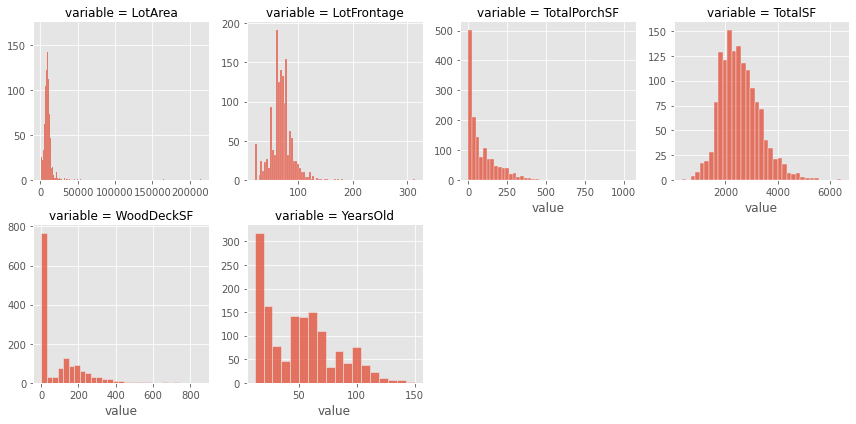
\includegraphics[width=\textwidth]{skewplots}
		\caption{Histograms for the features. Lot Area, Lot Frontage, Total Porch Square Footage, Total Square Footage, Wood Deck Square Footage, and Years Old. Their skew values are 1.54, 12.59, 1.55, 0.65, 2.01, and 0.61, respectively.}
		\label{fig:skew}
	\end{figure}
	
	Finally we have our target variable. Sale Price for the house is our target variable, as that is the ultimate outcome when looking at all the variables together. It is a pretty self explanatory variable being the price the house was sold at, as a numerical variable. Since it is our target, we want to inspect it more closely and better understand and prepare it for analysis. We can see from the bar chart that the sale price is pretty heavily skewed to the right and will need some adjustments to be made. In order to get it to a normal distribution we will log transform Sales Price.

	%...

\begin{figure}[h!]
	\centering
	\begin{subfigure}[b]{0.4\linewidth}
	  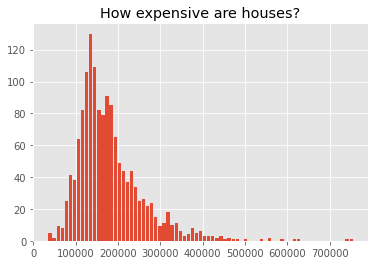
\includegraphics[width=\linewidth]{salehist}
	  \caption{A histogram of the target variable, Sale Price}
	\end{subfigure}
	\begin{subfigure}[b]{0.4\linewidth}
	  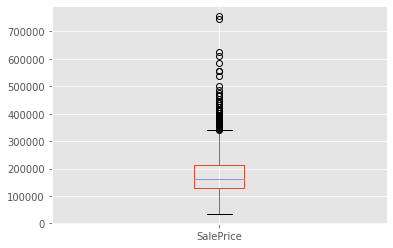
\includegraphics[width=\linewidth]{salebox}
	  \caption{A box plot of the target variable, Sale Price. }
	\end{subfigure}
	\caption{Notice the outliers in upper ranges.}
	\label{fig:saleprice}
  \end{figure}
  
  %...

  \subsection{Correlation of Variables}
	
	We then take a look at some different correlations with sale price and with all the other features. With the correlation to just sales price we see that Total Square Footage is the most positive correlated feature and Years Old is the highest negative correlated feature. This is starting to confirm what we believe and shows that Age and Size have the biggest impact on sale price. When looking at the correlation matrix, we see Total Square Footage and Total Rooms Above Ground, and Total Baths and Total Square footage are the most highly correlated features. This would make sense as the more rooms there are, the higher the square footage will be. The same holds for Total baths and square footage, as the more bathrooms the more space in the house there will be. From this, since Bathroom Square Footage is not included in Total Square Footage we will keep it, and remove Total Rooms Above Ground. These are the correlation graphs:
	
	%...

	\begin{figure}[h!]
		\centering
		\begin{subfigure}[b]{0.4\linewidth}
		  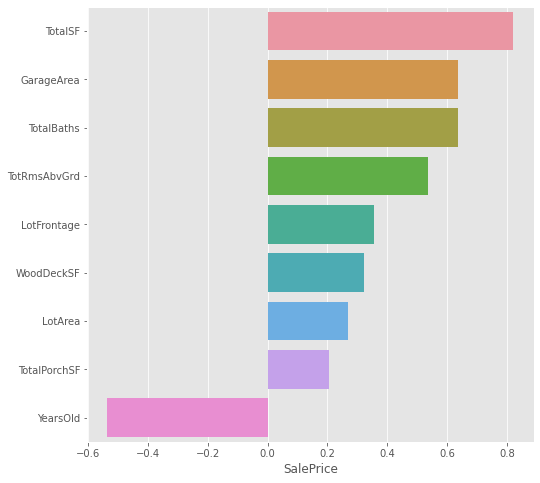
\includegraphics[width=\linewidth]{salecorr}
		  \caption{A bar plot of correlation coefficients of numerical variables to the target variable, Sale Price.}
		\end{subfigure}
		\begin{subfigure}[b]{0.4\linewidth}
		  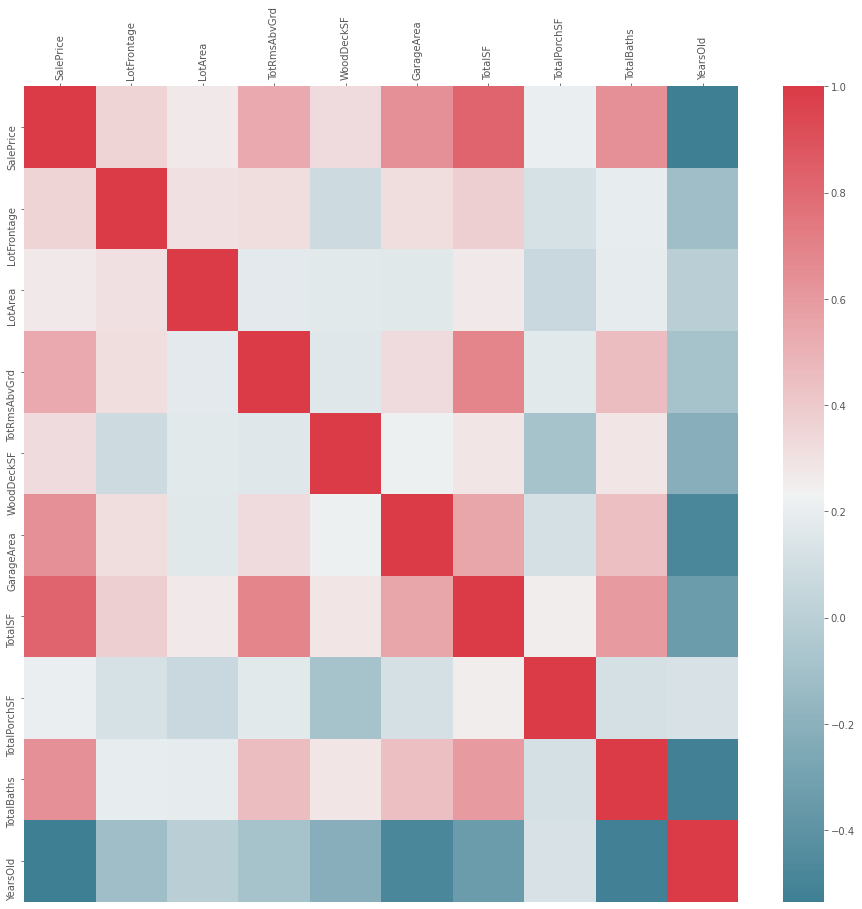
\includegraphics[width=\linewidth]{corrmatrix}
		  \caption{A correlation matrix of all numerical variables in the dataset.}
		\end{subfigure}
		\label{fig:correlation}
	  \end{figure}
	  
	  %...
	

	\subsection{Analysis of Categorical Variables}

	Looking at the categorical we plot the averages against each other to get a visual idea of whats going on. Visually looking at the plots, we see that Neighborhood and Overall Quality look to have statistically significant different means. 
	
	\begin{figure}
		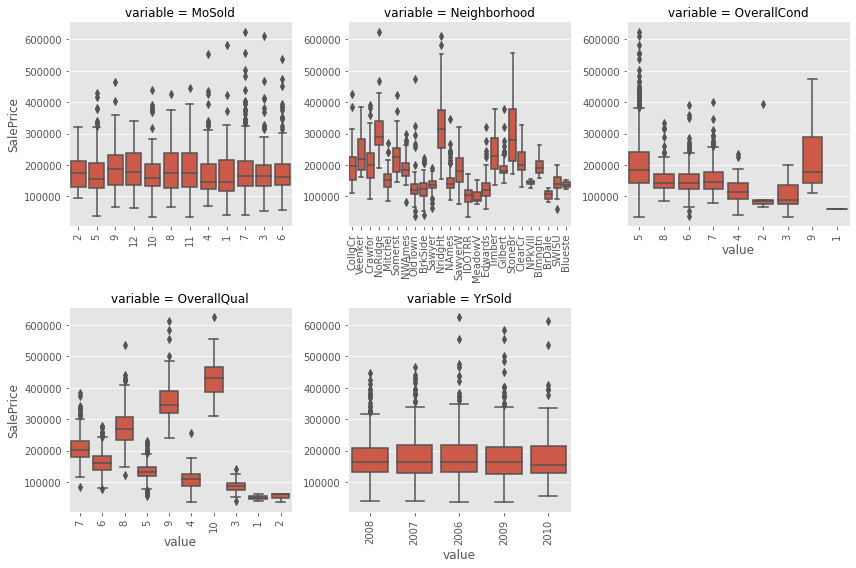
\includegraphics[width=\textwidth]{catboxes}
		\caption{Box Plots of all categorical variables. Neighborhood, Overall Qual, and Overall Condition have noticably different means.}
		\label{fig:cats}
	\end{figure}
	
	Since it appears so, we will run an ANOVA test to truly determine if our categorical values are different. After running ANOVA on all our variables we see that the only features that do not have different means are Month Sold and Year Sold. Since they do not have different means we will remove them as they have no impact. 
	
	\begin{table}[]
		\centering
		\begin{tabular}{llll}
		\hline
		\multicolumn{1}{|l|}{Feature} & \multicolumn{1}{l|}{F-Stat} & \multicolumn{1}{l|}{P-value} & \multicolumn{1}{l|}{Significant?} \\ \hline
		Overall Quality               & 374.11                      & 0.00                         & True                              \\
		Neighborhood                  & 74.02                       & 1.63e-230                    & True                              \\
		Overall Condition             & 28.84                       & 1.87e-41                     & True                              \\
		Month Sold                    & 0.98                        & 0.458                        & False                             \\
		Year Sold                     & 0.32                        & 0.865                        & False                            
		\end{tabular}
		\end{table}
	

	Overall Quality, Neighborhoods and Overall Condition do have significantly different means and therefore they may have an impact and we will have to keep them in for analysis.
	
	
	First look at data / pre-processing
	
	exploratory methods
	
	maybe final method
	
	
	\section{Results}
	
	
	maybe discussion as its own section?
	
	
	\section{Conclusion}
	
	
\end{document}